\section{AFD Paridad en números binarios}
	\subsection{Descripción del problema}
	Diseñar y programar un autómata finito determinista que acepte el lenguaje:
	\[ L = \lbrace w \mid w \text{ tiene un número par de ceros y un numero par de unos} \rbrace \text{\cite{LIBRO}}\] 
	Es decir, los números binarios de entrada se generan de manera automática (cadena de longitud $n \mid 1\leq n \leq 1000$) o manual y después se imprime si es una cadena valida o no y en ambos casos imprimir su historia. Ademas, mostrar el siguiente diagrama.
	\begin{figure}[ht]
		\begin{center}
			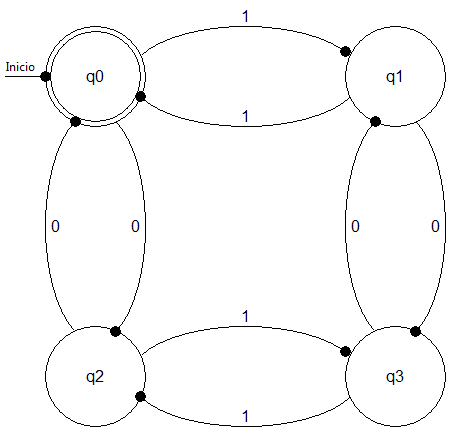
\includegraphics[width=7cm, height=7cm]{img/paridad.png}
			\caption{Diagrama de transiciones del autómata. \cite{LIBRO}}
			\label{fig:diagrama2}
		\end{center}
	\end{figure}
	\subsection{Código}
	El código fue realizado en Python 3.5.
	\subsection{Pruebas}
	Pruebas de las opciones del menú.
	{\large Modo automático.}
	{\large Modo manual.}
	{\large Diagrama.}